\chapter{RDF -- the basis of the Semantic Web}
\label{ch3}
RDF, RDFS, and OWL are the basic representation languages of the
Semantic Web, with RDF serving as the foundation. RDF addresses one
fundamental issue in the Semantic Web: managing distributed data. All
other Semantic Web standards build on this foundation of distributed
data. RDF relies heavily on the infrastructure of the Web, using many of
its familiar and proven features, while extending them to provide a
foundation for a distributed network of data and the resulting paradigm
of linked data on the Web will be explained in details in Chapter~\ref{ch5}.

The Web that we are accustomed to is made up of hypertext documents that are
linked to one another. Any connection between a document and the
thing(s) in the world it describes is made only by the person who reads
it. There could be a link from a document about Shakespeare to
a document about Stratford-upon-Avon, but there is no notion of an
entity that is Shakespeare or linking it to the thing that is Stratford.

In the Semantic Web we refer to the things in the world as resources; a
resource can be anything that someone might want to talk about. Shakespeare, Stratford, ``the
value of X,'' and ``all the cows in Texas'' are all examples of things
someone might talk about and that can be resources in the Semantic Web.
This is admittedly a pretty odd use of the word resource, but
alternatives like entity or thing, which might be more accurate, have
their own issues. In any case, resource is the word used in the
Semantic Web standards. In fact, the name of the base technology in the
Semantic Web (RDF) uses this word in an essential way: RDF stands for
Resource Description Framework.

In a web of information, anyone can contribute to our knowledge about a
resource. It was this aspect of the current Web that allowed it to grow
at such an unprecedented rate. To implement the Semantic Web, we need a
model of data that allows information to be distributed over the Web.

\section{Distributing Data Across the Web}

Data are most often represented in tabular form, in which each row
represents some item we are describing, and each column represents some
property of those items. The cells in the table are the particular
values for those properties. Table~\ref{tab:ch3.1} shows a sample of some data about
works completed around the time of Shakespeare.

Let's consider a few different strategies for how these data could be
distributed over the Web. In all of these strategies, some part of the
data will be represented on one computer, while other parts will be
represented on another. Figure~\ref{fig:ch3.1} shows one strategy for distributing
information over many machines. Each networked machine is responsible
for maintaining the information about one or more complete rows from the
table. Any query about an entity can be answered by the machine that
stores its corresponding row. One machine is responsible for information
about \emph{Sonnet 78} and \emph{Edward II}, whereas another is
responsible for information about \emph{As You Like It}.

This distribution solution provides considerable flexibility, since the
machines can share the load of representing information about several
individuals. But because it is a distributed representation of data, it
requires some coordination between the servers. In particular, each
server must share information about the columns. Does the second column
on one server correspond to the same information as the second column on
another server? This is not an insurmountable problem, and, in fact, it
is a fundamental problem of data distribution. There must be some
agreed-on coordination between the servers. In this example, the servers
must be able, in a global way, to indicate which property each column
corresponds to.

\begin{table}[h]
\centering
\begin{tabular}{||l l l l l||} 
 \hline
 ID & Title & Author & Medium & Year \\ [0.5ex] 
 \hline\hline
1&As You Like It&Shakespeare&Play&1599\\
2&Hamlet&Shakespeare&Play&1604\\
3&Othello&Shakespeare&Play&1603\\
4&``Sonnet 78''&Shakespeare&Poem&1609\\
5&Astrophil and Stella&Sir Phillip Sidney&Poem&1590\\
6&Edward II&Christopher Marlowe&Play&1592\\
7&Hero and Leander&Christopher Marlowe&Poem&1593\\
8&Greensleeves&Henry VIII Rex&Song&1525\\
\hline
\end{tabular}
\caption{Tabular Data about Elizabethan Literature and Music}
\label{tab:ch3.1}
\end{table}


\begin{figure}
    \centering
    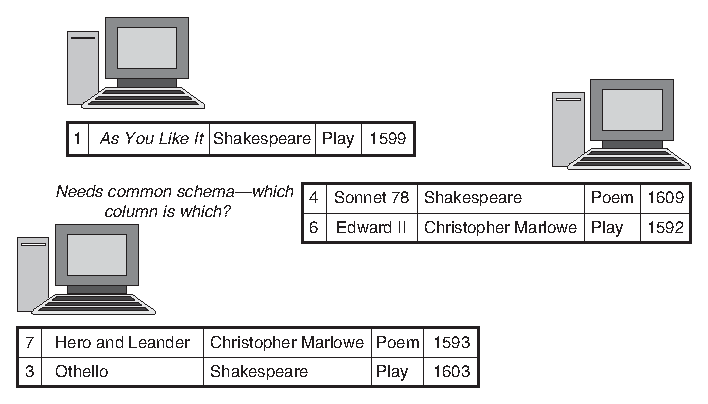
\includegraphics[width=5.0in]{media/ch3/f03-01-9780123859655.eps}
    \caption{Distributing data across the Web, row by row.}
    \label{fig:ch3.1}
\end{figure}



\begin{figure}
    \centering
    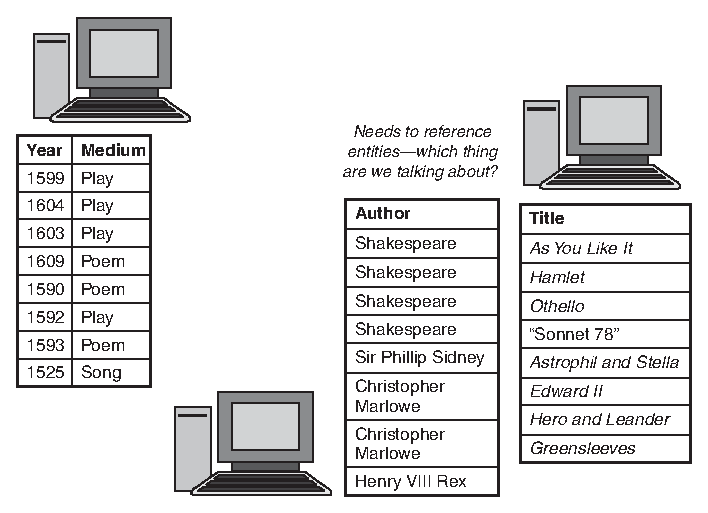
\includegraphics[width=5.0in]{media/ch3/f03-02-9780123859655.eps}
    \caption{Distributing data across the Web, column by column.}
    \label{fig:ch3.2}
\end{figure}



\begin{figure}
    \centering
    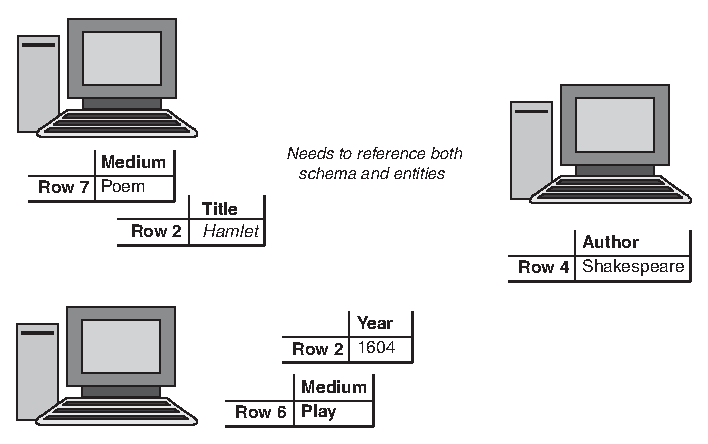
\includegraphics[width=5.0in]{media/ch3/f03-03-9780123859655.eps}
    \caption{Distributing data across the Web, cell by cell.}
    \label{fig:ch3.3}
\end{figure}



Figure~\ref{fig:ch3.2} shows another strategy, in which each server is responsible
for one or more complete columns from the original table. In this
example, one server is responsible for the publication dates and medium,
and another server is responsible for titles. This solution is flexible
in a different way from the solution of Figure~\ref{fig:ch3.1}. The solution in
Figure~\ref{fig:ch3.2} allows each machine to be responsible for one kind of
information. If we are not interested in the dates of publication, we
needn't consider information from that server. If we want to specify
something new about the entities (say, how many pages the manuscript
is), we can add a new server with that information without disrupting
the others.

This solution is similar to the solution in Figure 3.1 in that it
requires some coordination between the servers. In this case, the
coordination has to do with the identities of the entities to be
described. How do I know that row 3 on one server refers to the same
entity as row 3 on another server? This solution requires a global
identifier for the entities being described.

The strategy outlined in Figure~\ref{fig:ch3.3} is a combination of the previous two
strategies, in which information is neither distributed row by row nor
column by column but instead is distributed cell by cell. Each machine
is responsible for some number of cells in the table. This system
combines the flexibility of both of the previous strategies. Two servers
can share the description of a single entity (in the figure, the year
and title of Hamlet are stored separately), and they can share the use
of a particular property (in Figure~\ref{fig:ch3.3}, the Medium of rows 6 and 7 are
represented on different servers).

This flexibility is required if we want our data distribution system to
really support the AAA slogan that ``Anyone can say Anything about Any topic.'' If we take the AAA
slogan seriously, any server needs to be able to make a statement about
any entity (as is the case in Figure~\ref{fig:ch3.2}), but also any server needs to
be able to specify any property of an entity (as is the case in Figure~\ref{fig:ch3.1}). The solution in Figure~\ref{fig:ch3.3} has both of these benefits.


\begin{table}[h]
\centering
\begin{tabular}{||l l l||} 
 \hline
Subject&Predicate&Object \\ [0.5ex] 
 \hline\hline
Row 7&Medium&Poem \\
Row 2&Title&Hamlet \\
Row 2&Year&1604\\
Row 4&Author&Shakespeare\\
Row 6&Medium&Play\\

\hline
\end{tabular}
\caption{Sample triples}
\label{tab:ch3.2}
\end{table}





But this solution also combines the costs of the other two strategies.
Not only do we now need a global reference for the column headings, but
we also need a global reference for the rows. In fact, each cell has to
be represented with three values: a global reference for the row, a
global reference for the column, and the value in the cell itself. This
third strategy is the strategy taken by RDF. We will see how RDF
resolves the issue of global reference later in this chapter, but for
now, we will focus on how a table cell is represented and managed in
RDF.

Since a cell is represented with three values, the basic building block
for RDF is called the \emph{triple}. The identifier for the row is called the
\emph{subject} of the triple (following the notion from elementary grammar,
since the subject is the thing that a statement is about). The
identifier for the column is called the \emph{predicate} of the triple (since
columns specify properties of the entities in the rows). The value in
the cell is called the \emph{object} of the triple. Table~\ref{tab:ch3.2} shows the triples
in Figure~\ref{fig:ch3.3} as subject, predicate, and object.

Triples become more interesting when more than one triple refers to the
same entity, such as in Table~\ref{tab:ch3.3}. When more than one triple refers to
the same thing, sometimes it is convenient to view the triples as a
directed graph in which each triple is an edge from its subject to its
object, with the predicate as the label on the edge, as shown in Figure~\ref{fig:ch3.4}. The graph visualization in Figure~\ref{fig:ch3.4} expresses the same
information presented in Table~\ref{tab:ch3.3}, but everything we know about
Shakespeare (either as subject or object) is displayed at a single node.

\begin{table}[h]
\centering
\begin{tabular}{||l l l||} 
 \hline
 Subject&Predicate&Object \\ [0.5ex] 
 \hline\hline
Shakespeare&wrote&King Lear \\
Shakespeare&wrote&Macbeth \\
Anne Hathaway&married&Shakespeare \\
Shakespeare&livedIn&Stratford \\
Stratford&isIn&England\\
Macbeth&setIn&Scotland\\
England&partOf&UK \\
Scotland&partOf&UK \\
\hline
\end{tabular}
\caption{Sample triples}
\label{tab:ch3.3}
\end{table}




\begin{figure}
    \centering
    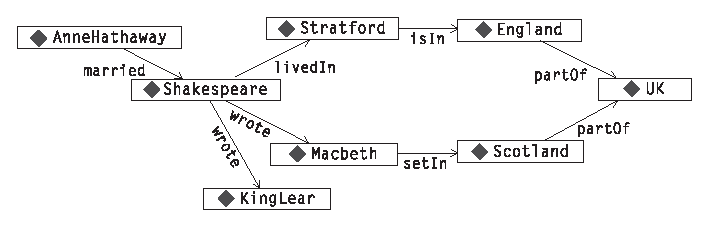
\includegraphics[width=5.0in]{media/ch3/f03-04-9780123859655.eps}
    \caption{Graph display of triples from Table \ref{tab:ch3.3}. Eight triples appear as eight labeled edges.}
    \label{fig:ch3.4}
\end{figure}


\section{MERGING DATA FROM MULTIPLE SOURCES}

We started off describing RDF as a way to distribute data over several
sources. But when we want to use that data, we will need to merge those
sources back together again. One value of the triples representation is
the ease with which this kind of merger can be accomplished. Since
information is represented simply as triples, merged information from
two graphs is as simple as forming the graph of all of the triples from
each individual graph, taken together. Let's see how this is
accomplished in RDF.

Suppose that we had another source of information that was relevant to
our example from Table~\ref{tab:ch3.3}---that is, a list of plays that Shakespeare wrote or a list of parts
of the United Kingdom. These would be represented as triples as in
Tables~\ref{tab:ch3.4} and \ref{tab:ch3.5}. Each of these can also be shown as a graph, just as
in the original table, as shown in Figure~\ref{fig:ch3.5}.

What happens when we merge together the information from these three
sources? We simply get the graph of all the triples that show up in
Figures \ref{fig:ch3.4} and \ref{fig:ch3.5}. Merging graphs like those in Figures \ref{fig:ch3.4} and \ref{fig:ch3.5} to
create a combined graph like the one shown in Figure~\ref{fig:ch3.6} is a
straightforward process---but only when it is known which nodes in each
of the source graphs match.

\begin{table}[h]
\centering
\begin{tabular}{||l l l||} 
 \hline
 Subject&Predicate&Object \\ [0.5ex] 
 \hline\hline
Scotland&part Of&The UK \\
England&part Of&The UK \\
Wales&part Of&The UK\\
Northern Ireland&part Of&The UK \\
Channel Islands&part Of&The UK\\
Isle of Man&part Of&The UK\\
\hline
\end{tabular}
\caption{Triples about the Parts of the United Kingdom}
\label{tab:ch3.5}
\end{table}

\begin{table}[h]
\centering
\begin{tabular}{||l l l||} 
 \hline
 Subject&Predicate&Object \\ [0.5ex] 
 \hline\hline
Shakespeare&wrote&As You Like It\\
Shakespeare&wrote&Henry V\\
Shakespeare&wrote&Love's Labour's Lost \\
Shakespeare&wrote&Measure for Measure \\
Shakespeare&wrote&Twelfth Night \\
Shakespeare&wrote&The Winter's Tale \\
Shakespeare&wrote&Hamlet\\
Shakespeare&wrote&Othello\\
\hline
\end{tabular}
\caption{Triples about Shakespeare's Plays}
\label{tab:ch3.4}
\end{table}


\begin{figure}
    \centering
    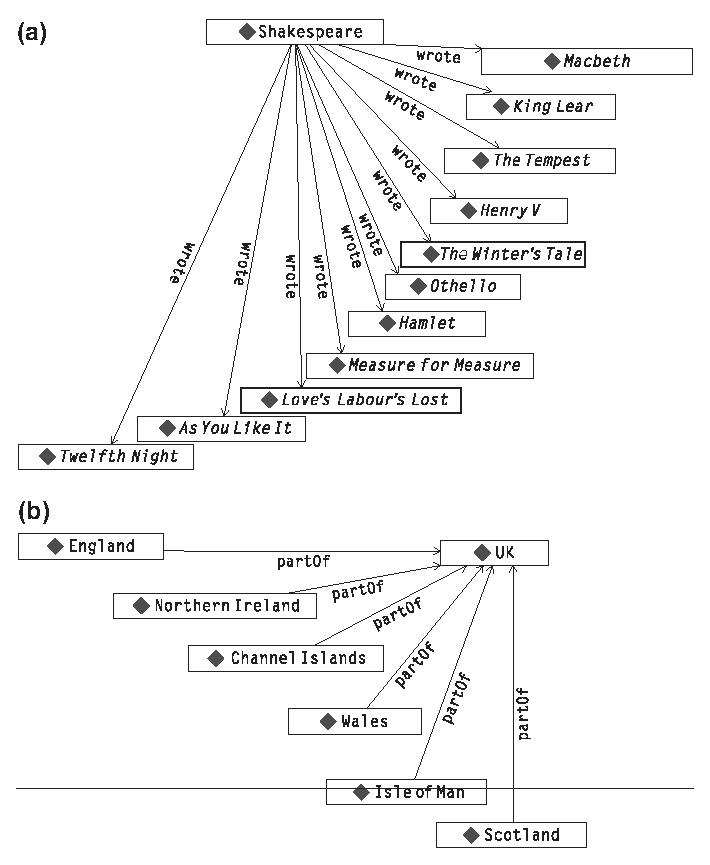
\includegraphics[width=5.0in]{media/ch3/f03-05ab-9780123859655.eps}
    \caption{Graphic representation of triples describing (a) Shakespeare’s plays and (b) parts of the United Kingdom.}
    \label{fig:ch3.5}
\end{figure}


\begin{figure}
    \centering
    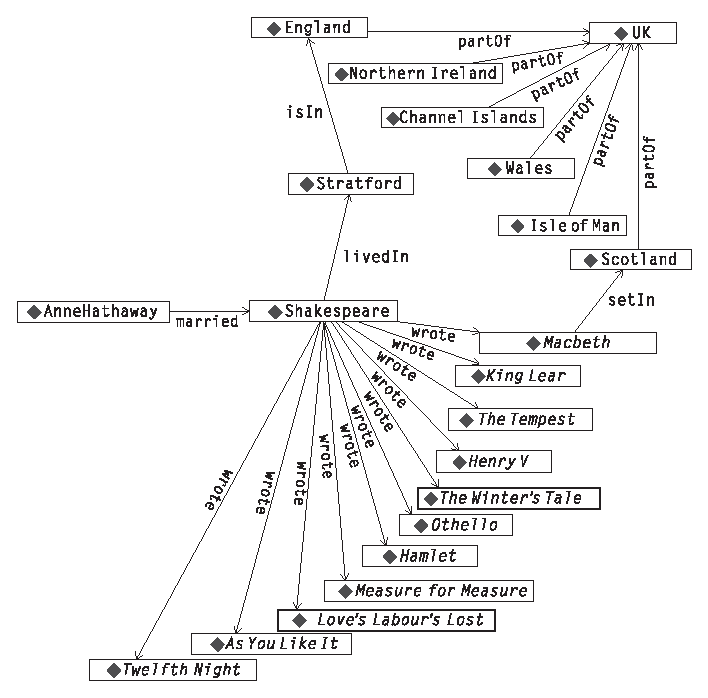
\includegraphics[width=5.0in]{media/ch3/f03-06-9780123859655.eps}
    \caption{Combined graph of all triples about Shakespeare and the United Kingdom.}
    \label{fig:ch3.6}
\end{figure}



\section{Namespaces, Uris, and Identity}

The essence of the merge process comes down to answering the question ``When is
a node in one graph the same node as a node in another graph?'' In RDF,
this issue is resolved through the use of Uniform Resource Identifiers
(URIs).

In the figures so far, we have labeled the nodes and edges in the graphs
with simple names like Shakespeare or Wales. On the Semantic Web, this
is not sufficient information to determine whether two nodes are really
the same. Why not? Isn't there just one thing in the universe that
everyone agrees refers to as Shakespeare? When referring to agreement on
the Web, never say, ``everyone.'' Some- where, someone will refer not to
the historical Shakespeare but to the title character of the feature
film \emph{Shakespeare in Love}, which bears very little resemblance to
the historical figure. And ``Shakespeare'' is one of the more stable
concepts to appear on the Web; consider the range of referents for a
name like ``Washington'' or ``Bordeaux.'' To merge graphs in a Semantic
Web setting, we have to be more specific: In what sense do we mean the
word Shakespeare?

RDF borrows its solution to this problem from foundational Web
technology --- in particular, the URI. The syntax and format of a URI are
familiar even to casual users of the Web today because of the special,
but typical, case of the URL --- for example,
{http://www.workingontologist.org/Examples/Chapter3/Shakespeare\#Shakespeare}. 
But the significance of the URI as a
global identifier for a Web resource is often not appreciated. A URI
provides a global identification for a resource that is common across
the Web. This is not a stipulation that is particular to the Semantic
Web but to the Web in general; global naming leads to global network
effects. Of course, in the jungle that is the web, we can't expect that
every data source that refers to Shakespeare will use the same URI In
Chapter~\ref{ch5} we will explore when and why we might use different URIs for
the same individual, and what capabilities the Semantic Web provides to
manage them.

URIs and URLs look exactly the same, and, in fact, a URL is just a
special case of the URI. Why does the Web have both of these ideas?
Simplifying somewhat, the URI is an identifier with global (i.e.,
``World Wide'' in the ``World Wide Web'' sense) scope. Any two Web
applications in the world can refer to the same thing by referencing the
same URI. But the syntax of the URI makes it possible to ``dereference''
it---that is, to use all the information in the URI (which specifies
things like server name, protocol, port number, file name, etc.) to
locate a file (or a location in a file) on the Web \footnote{We are primarily discussing files here, but a URI can refer to other
resources. The Wikipedia article on URIs includes more than 50 different
resource types that can be referenced by URIs---see
\url{http://en.wikipedia.org/wiki/URI_} scheme.}. This
dereferencing succeeds if all these parts work; the protocol locates the
specified server running on the specified port and so on. When this is
the case, we can say that the URI is not just a URI, but an effective
HTTP URI. From the point of view of modeling, the distinction is not
important. But from the point of view of having a model on the Semantic
Web, the fact that a URI can potentially be dereferenced allows the
models to participate in a global Web infrastructure as we will see in
chapter~\ref{ch5}

RDF applies the notion of the URI to resolve the identity problem in
graph merging. The application is quite simple: A node from one graph is
merged with a node from another graph exactly if they have the same
URI. On the one hand, this may seem disingenuous, ``solving'' the
problem of node identity by relying on another standard to solve it. On
the other hand, since issues of identity appear in the Web in general
and not just in the Semantic Web, it would be foolish not to use the
same strategy to resolve the issue in both cases.

\subsection{Expressing URIs in print}

URIs work very well for expressing identity on the World Wide Web, but
they are typically a bit of a pain to write out in detail when
expressing models, especially in print. So for the examples in this
book, we use a simplified version of a URI abbreviation scheme called
\emph{QNames} (standing for \emph{qualified names}). In its simplest form, a
URI expressed as a QName has two parts: a namespace and an identifier,
written with a colon between. So the QName representation for the
identifier \emph{England} in the namespace \emph{geo} is simply \texttt{geo:England}.
The RDF standard syntaxes include elaborate rules that allow programmers
to map namespaces to other URI representations (such as the familiar
\emph{http://} notation). For the examples in this book, we will use the
simple QName form for all URIs. It is important, however, to note that
QNames are \emph{not} global identifiers on the Web; only fully
qualified URIs (e.g.
\emph{http://www.WorkingOntologist.org/Examples/Chapter3/Shakespeare\#Shakespeare})
are global Web names. Thus, any representation of a QName must, in
principle, be accompanied by a declaration of the namespace
correspondence.

It is customary on the Web in general and part of the XML specification
to insist that URIs contain no embedded spaces. For example, an
identifier ``part of'' is typically not used in the web. Instead, we
follow the InterCap convention (sometimes called CamelCase), whereby
names that are made up of multiple words are transformed into
identifiers without spaces by capitalizing each word. Thus, ``part of''
becomes partOf, ``Great Britain'' becomes GreatBritain, ``Measure for
Measure'' becomes MeasureForMeasure, and so on.

There is no limitation on the use of multiple namespaces in a single
source of data, or even in
a single triple. Selection of namespaces is entirely unrestricted as far
as the data model and standards are concerned. It is common practice,
however, to refer to related identifiers in a single namespace. For
instance, all of the literary or geographical information from Table~\ref{tab:ch3.4}
or Table~\ref{tab:ch3.5} would be placed into one namespace per table, with a
suggestive name---say, \emph{lit} or \emph{geo}---respectively. Strictly
speaking, these names correspond to fully qualified URIs---for example,
\emph{lit} stands for \emph{http://www.WorkingOntologist.com/Examples/Chapter3/Shakespeare\#}, and
\emph{geo} stands for \emph{http://www.WorkingOntologist.com/Examples/Chapter3/geography\#}.


For the purposes of explaining modeling on the Semantic Web, the
detailed URIs behind the QNames are not important, so for the most part,
we will omit these bindings from now on. In many examples, we will take
this notion of abbreviation one step further; in the cases when we use a
single namespace throughout one example, we will assume there is a
default namespace declaration that allows us to refer to URIs simply
with a symbolic name preceded by a colon (:), such as :Shakespeare,
:JamesDean, :Researcher.

\begin{table}[h]
\centering
\begin{tabular}{||l l l ||} 
 \hline
 Subject&Predicate&Object \\ [0.5ex] 
 \hline\hline
lit:Shakespeare&lit:wrote&lit:AsYouLikeIt\\
lit:Shakespeare&lit:wrote&lit:HenryV\\
lit:Shakespeare&lit:wrote&lit:LovesLaboursLost\\
lit:Shakespeare&lit:wrote&lit:MeasureForMeasure\\
lit:Shakespeare&lit:wrote&lit:TwelfthNight\\
lit:Shakespeare&lit:wrote&lit:WintersTale\\
lit:Shakespeare&lit:wrote&lit:Hamlet\\
lit:Shakespeare&lit:wrote&lit:Othello\\
\hline
\end{tabular}
\caption{Plays of Shakespeare with QNames}
\label{tab:ch3.6}
\end{table}



\begin{table}[h]
\centering
\begin{tabular}{||l l l ||} 
 \hline
 Subject&Predicate&Object \\ [0.5ex] 
 \hline\hline
geo:Scotland&geo:partOf&geo:UK \\
geo:England&geo:partOf&geo:UK \\
geo:Wales&geo:partOf&geo:UK \\
geo:NorthernIreland&geo:partOf&geo:UK \\
geo:ChannelIslands&geo:partOf&geo:UK \\
geo:IsleOfMan&geo:partOf&geo:UK \\
\hline
\end{tabular}
\caption{Geographical names with QNames}
\label{tab:ch3.7}
\end{table}

Using QNames, our triple sets now look as shown in Tables~\ref{tab:ch3.6} and \ref{tab:ch3.7}.
Compare Table~\ref{tab:ch3.6} with Table~\ref{tab:ch3.4}, and compare Table~\ref{tab:ch3.7} with Table~\ref{tab:ch3.5}.
But it isn't always that simple; some triples will have to use
identifiers with different namespaces, as in the example in Table~\ref{tab:ch3.8},
which was taken from Table~\ref{tab:ch3.3}.

In Table~\ref{tab:ch3.8}, we introduced a new namespace, \emph{bio:}, without
specifying the actual URI to which it corresponds. For this model to
participate on the Web, this information must be filled in. But from the
point of view of modeling, this detail is unimportant. For the rest of
this book, we will assume that the prefixes of all QNames are defined,
even if that definition has not been specified explicitly in print.

\subsection{Standard namespaces}

Using the URI as a standard for global identifiers allows for a
worldwide reference for any symbol. This means that we can tell when any
two people anywhere in the world are referring to the same thing.

This property of the URI provides a simple way for a standard
organization (like the W3C) to specify the meaning of certain terms in
the standard. As we will see in coming chapters, the W3C standards
provide definitions for terms such as type, subClassOf, Class,
inverseOf, and so forth. But these standards are intended to apply
globally across the Semantic Web, so the standards

\begin{table}[h]
\centering
\begin{tabular}{||l l l ||} 
 \hline
 Subject&Predicate&Object \\ [0.5ex] 
 \hline\hline
lit:Shakespeare&lit:wrote&lit:KingLear\\
lit:Shakespeare&lit:wrote&lit:MacBeth\\
bio:AnneHathaway&bio:married&lit:Shakespeare\\
bio:AnneHathaway&bio:livedWith&lit:Shakespeare\\
lit:Shakespeare&bio:livedIn&geo:Stratford\\
geo:Stratford&geo:isIn&geo:England\\
geo:England&geo:partOf&geo:UK\\
geo:Scotland&geo:partOf&geo:UK\\
\hline
\end{tabular}
\caption{Triples Referring to URIs with a Variety of Namespaces}
\label{tab:ch3.8}
\end{table}

refer to these reserved words in the same way as they refer to any other
resource on the Semantic Web, as URIs.

The W3C has defined a number of standard namespaces for use with Web
technologies, including \emph{xsd:} for XML schema definition;
\emph{xmlns:} for XML namespaces; and so on. The Semantic Web is handled
in exactly the same way, with namespace definitions for the major layers
of the Semantic Web. Following standard practice with the W3C, we will
use QNames to refer to these terms, using the following definitions for
the standard namespaces.

\emph{rdf}: Indicates identifiers used in RDF. The set of identifiers defined
in the standard is quite small and is used to define types and
properties in RDF. The global URI for the rdf namespace is http://
\href{http://www.w3.org/1999/02/22-rdf-syntax-ns}{www.w3.org/1999/02/22-rdf-syntax-ns\#.}

\emph{rdfs}: Indicates identifiers used for the RDF Schema language, RDFS. The
scope and semantics of the symbols in this namespace are the topics of
future chapters. The global URI for the rdfs namespace is
\href{http://www.w3.org/2000/01/rdf-schema}{http://www.w3.org/2000/01/rdf-schema\#.}

\emph{owl}: Indicates identifiers used for the Web Ontology Language, OWL. The
scope and semantics of the symbols in this namespace are the topics of
future chapters. The global URI for the owl namespace is
\href{http://www.w3.org/2002/07/owl}{http://www.w3.org/2002/07/owl\#.}

These URIs provide a good example of the interaction between a URI and a
URL. For modeling purposes, any URI in one of these namespaces (e.g.,
\emph{http://www.w3.org/2000/01/rdf-schema\#subClassOf}, or
\texttt{rdfs:subClassOf} for short) refers to a particular term that the W3C
makes some statements about in the RDFS standard. But the term can also
be dereferenced---that is, if we look at the server
www.w3.org, there is a page at the location
2000/01/rdf-schema with an entry about subClassOf, giving supplemental
information about this resource. From the point of view of modeling, it
is not necessary that it be possible to dereference this URI, but from
the point of view of Web integration, it is critical that it is. The
underlying standards and principles to weave such a Web of linked data
will be detailed in chapter~\ref{ch5}.
% Check this once you read ch 5

\section{Identifiers in the RDF Namespace}

The RDF data model specifies the notion of triples and the idea of
merging sets of triples as just shown. With the introduction of
namespaces, RDF uses the infrastructure of the Web to represent
agreements on how to refer to a particular entity. The RDF standard itself takes
advantage of the namespace infrastructure to define a small number of
standard identifiers in a namespace defined in the standard, a namespace
called rdf.


\begin{table}[h]
\centering
\begin{tabular}{||l l l ||} 
 \hline
 Subject&Predicate&Object \\ [0.5ex] 
 \hline\hline
lit:Shakespeare&rdf:type&lit:Playwright \\
lit:Ibsen&rdf:type&lit:Playwright \\
lit:Simon&rdf:type&lit:Playwright \\
lit:Miller&rdf:type&lit:Playwright \\
lit:Marlowe&rdf:type&lit:Playwright \\
lit:Wilder&rdf:type&lit:Playwright \\
\hline
\end{tabular}
\caption{Using rdf:type to Describe Playwrights}
\label{tab:ch3.9}
\end{table}


\begin{table}[h]
\centering
\begin{tabular}{||l l l ||} 
 \hline
 Subject&Predicate&Object \\ [0.5ex] 
 \hline\hline
lit:Playwright&rdf:type&bus:Profession \\
bus:Profession&rdf:type&hr:Compensation \\
\hline
\end{tabular}
\caption{Defining Types of Names}
\label{tab:ch3.10}
\end{table}



\texttt{rdf:type} is a property that provides an elementary typing system in RDF.
For example, we can express the relationship between several playwrights
using type information, as shown in Table~\ref{tab:ch3.9}. The subject of \texttt{rdf:type}
in these triples can be any identifier, and the object is understood to
be a type. There is no restriction on the usage of \texttt{rdf:type}
with types;
types can have types ad infinitum, as shown in Table~\ref{tab:ch3.10}.

When we read a triple out loud (or just to ourselves), it is
understandably tempting to read it (in English, anyway) in
subject/predicate/object order so that the first triple in Table~\ref{tab:ch3.9}
would read, ``Shakespeare type Playwright.'' Unfortunately, this is
pretty fractured syntax no matter how you inflect it. It would be better
to have something like ``Shakespeare has type Playwright'' or maybe
``The type of Shakespeare is Playwright.''

This issue really has to do with the choice of name for the \texttt{rdf:type}
resource; if it had been called rdf:isInstanceOf instead, it would have
been much easier to read out loud in English. But since we never have
control over how other entities (in this case, the W3C) chose their
names, we don't have the luxury of changing these names. When we read
out loud, we just have to take some liberties in adding in connecting
words. So this triple can be pronounced, ``Shakespeare {[}has{]} type
Playwright,'' adding in the ``has'' (or sometimes, the word ``is'' works
better) to make the sentence into somewhat correct English. Later in
this chapter, we'll see the Turtle syntax for writing RDF, in which a
shortcut has been introduced for this particular case: the keyword ``a''
can be used instead of rdf:type which makes the reading ever easier
``Shakespeare {[}is{]} a Playwright''.

\texttt{rdf:Property} is an identifier that is used as a type in RDF to indicate
when another identifier is to be used as a predicate rather than as a
subject or an object. We can declare all the identifiers we have used as
predicates so far in this chapter as shown in Table~\ref{tab:ch3.11}.

\begin{table}[h]
\centering
\begin{tabular}{||l l l ||} 
 \hline
 Subject&Predicate&Object \\ [0.5ex] 
 \hline\hline
lit:wrote&rdf:type&rdf:Property\\
geo:partOf&rdf:type&rdf:Property\\
bio:married&rdf:type&rdf:Property\\
bio:livedIn&rdf:type&rdf:Property\\
bio:livedWith&rdf:type&rdf:Property\\
geo:isIn&rdf:type&rdf:Property\\
\hline
\end{tabular}
\caption{rdf:Property Assertions for Tables 3.5 to 3.8}
\label{tab:ch3.11}
\end{table}

\section{CHALLENGES: RDF and Tabular Data}

We began this chapter by motivating RDF as a way to distribute data over
the Web---in particular, tabular data. Now that we have all of the
detailed mechanisms of RDF (including namespaces and triples) in place,
we can revisit tabular data and show how to represent it consistently in
RDF.

\begin{challenge}
\label{chal:1}

Given a table from a relational database, describing products,
suppliers, and stocking information about the products (see Table~\ref{tab:ch3.12}),
produce an RDF graph that reflects its contents in such a
way that the information intent is preserved but the data are now
amenable for RDF operations like merging and RDF query.

\solution

Each row in the table describes a single entity, all of the same type.
That type is given by the name of the table itself, Product. We know
certain information about each of these items, based on the columns in
the table itself, such as the model number, the division, and so on. We
want to represent these data in RDF.

Since each row represents a distinct entity, each row will have a
distinct URI. Fortunately, the need for unique identifiers is just as present in the database as it is in the
Semantic Web, so there is a (locally) unique identifier
available---namely, the primary table key, in this case the column
called ID. For the Semantic Web, we need a globally unique identifier.
The simplest way to form such an identifier is by having a single URI
for the database itself (perhaps even a URL if the database is on the
Web). Use that URI as the namespace for all the identifiers in the
database. We will discuss the minting of URIs more in details in chapter~\ref{ch5}. 
Since this is a database for a manufacturing company, let's call that
namespace mfg:.

\begin{table}[h]
\centering
\begin{tabular}{||l l l l l l l ||} 
 \hline
 ID&Machine Number&Division&ProductLine&Manufacture Location&SKU&Available \\ [0.5ex] 
 \hline\hline
1&ZX-3&Manufacturing support&Papermachine&Sacramento&FB3524&23\\
2&ZX-3P&Manufacturing support&Paper machine&Sacramento&KD5243&4\\
3&ZX-3S&Manufacturing support&Paper machine&Sacramento&IL4028&34\\
4&B-1430&Control Engineering&Feedback line&Elizabeth&KS4520&23\\
5&B-1430X&Control Engineering&Feedback line&Elizabeth&CL5934&14\\
6&B-1431&Control Engineering&Active sensor&Seoul&KK3945&0\\
7&DBB-12&Accessories&Monitor&Hong Kong&ND5520&100\\
8&SP-1234&Safety&Safety valve&Cleveland&HI4554&4\\
9&SPX-1234&Safety&Safety valve&Cleveland&OP5333&14\\
\hline
\end{tabular}
\caption{Sample Tabular Data for Triples}
\label{tab:ch3.12}
\end{table}



Then we can create an identifier for each line by concatenating the
table name ``Product'' with the unique key and expressing this
identifier in the \emph{mfg:} namespace, resulting in identifiers \texttt{mfg:Product1},
\texttt{mfg:Product2}, and so on.

Each row in the table says several things about that item---namely, its
model number, its division, and so on. To represent this in RDF, each of these will be a property that will
describe the Products. But just as is the case for the unique
identifiers for the rows, we need to have global unique identifiers for
these properties. We can use the same namespace as we did for the
individuals, but since two tables could have the same column name (but
they aren't the same properties!), we need to combine the table name and
the column name. This results in properties like \texttt{mfg:Product\_ModelNo},
\texttt{mfg:Product\_Division}, and so on.

With these conventions in place, we can now express all the information
in the table as triples. There will be one triple per cell in the
table---that is, for n rows and c columns, there will be n x c triples.
The data shown in Table~\ref{tab:ch3.12} have 7 columns and 9 rows, so there are 63
triples, as shown in Table~\ref{tab:ch3.13}.

The triples in the table are a bit different from the triples we have
seen so far. Although the subject and  
predicate of these triples are RDF resources (complete with QName
namespaces!), the objects are not resources but literal data---that is,
strings, integers, and so forth. This should come as no surprise, since,
after all, RDF is a data representation system. RDF borrows from XML all
the literal data types as possible values for the object of a triple; in
this case, the types of all data are strings or integers.

The usual interpretation of a table is that each row in the table
corresponds to one individual and that the type of these individuals
corresponds to the name of the table. In Table~\ref{tab:ch3.12}, each row
corresponds to a Product. We can represent this in RDF by adding one
triple per row that specifies the type of the individual described by
each row, as shown in Table~\ref{tab:ch3.14}.

The full complement of triples from the translation of the information
in Table~\ref{tab:ch3.12} is shown in Figure~\ref{fig:ch3.7}. The types (i.e., where the
predicate is \texttt{rdf:type}, and the object is the class \texttt{mfg:Product}) are
shown as links in the graph; triples in which the object is a literal
datum are shown (for sake of compactness in the figure) within a box
labeled by their common subject.

\begin{table}[h]
\centering
\begin{tabular}{||l l l ||} 
 \hline
 Subject&Predicate&Object \\ [0.5ex] 
 \hline\hline
mfg:Product1&mfg:Product\_ID&1 \\
mfg:Product1&mfg:Product\_ModelNo&ZX-3 \\
mfg:Product1&mfg:Product\_Division&Manufacturing support \\
mfg:Product1&mfg:Product\_Product\_Line&Paper machine \\
mfg:Product1&mfg:Product\_Manufacture\_Location&Sacramento \\
mfg:Product1&mfg:Product\_SKU&FB3524 \\
mfg:Product1&mfg:Product\_Available&23 \\
mfg:Product2&mfg:Product\_ID&2\\
mfg:Product2&mfg:Product\_ModelNo&ZX-3P\\
mfg:Product2&mfg:Product\_Division&Manufacturing support \\
mfg:Product2&mfg:Product\_Product\_Line&Paper machine \\
mfg:Product2&mfg:Product\_Manufacture\_Location&Sacramento\\
mfg:Product2&mfg:Product\_SKU&KD5243\\
mfg:Product2&mfg:Product\_Available&4\\
\hline
\end{tabular}
\caption{Triples Representing Some of the Data in Table \ref{tab:ch3.12}}
\label{tab:ch3.13}
\end{table}

\begin{table}[h]
\centering
\begin{tabular}{||l l l ||} 
 \hline
 Subject&Predicate&Object \\ [0.5ex] 
 \hline\hline
mfg:Product1&rdf:type&mfg:Product\\
mfg:Product2&rdf:type&mfg:Product\\
mfg:Product3&rdf:type&mfg:Product\\
mfg:Product4&rdf:type&mfg:Product\\
mfg:Product5&rdf:type&mfg:Product\\
mfg:Product6&rdf:type&mfg:Product\\
mfg:Product7&rdf:type&mfg:Product\\
mfg:Product8&rdf:type&mfg:Product\\
mfg:Product9&rdf:type&mfg:Product\\
\hline
\end{tabular}
\caption{Triples Representing type information from Table \ref{tab:ch3.12}}
\label{tab:ch3.14}
\end{table}

\end{challenge}

\section{Higher-Order Relationships}

It is not unusual for someone who is building a model in RDF for the
first time to feel a bit limited by the simple subject/predicate/object
form of the RDF triple. They don't want to just say that Shakespeare
wrote Hamlet, but they want to qualify this statement and say that
Shakespeare wrote Hamlet in 1604 or that Wikipedia states that
Shakespeare wrote Hamlet in 1604. In general, these are cases in which
it is, or at least seems, desirable to make a statement about another
statement. This process is called \emph{reification}. Reification is not a
problem specific to Semantic Web modeling; the same issue arises in
other data modeling contexts like relational databases and object
systems. In fact, one approach to reification in the Semantic Web is to
simply borrow the standard solution that is commonly used in relational
database schemas, using the conventional mapping from relational tables
to RDF given in the preceding challenge. In a relational database table,
it is possible to simply create a table with more columns to add
additional information about a triple. So the statement
\emph{Shakespeare wrote Hamlet} is expressed (as in Table~\ref{tab:ch3.1}) in a
single row of a table, where there is a column for the author of a work
and another column for its title. Any further information about this
event is done with another column (again, just as in Table~\ref{tab:ch3.1}). When
this is converted to RDF according to the example in Challenge~\ref{chal:1}, the
row is represented by a number of triples, one triple per column in the
database. The subject of all of these triples is the same: a single
resource that corresponds to the row in the table.

An example of this can be seen in Table~\ref{tab:ch3.13}, where several triples have
the same subject and one triple apiece for each column in the table.
This approach to reification has a strong pedigree in rela-tional
modeling, and it has worked well for a wide range of modeling
applications. It can be applied in RDF even when the data have not been
imported from tabular form. That is, the statement \emph{Shakespeare
wrote Hamlet in 1601} (disagreeing with the statement in Table~\ref{tab:ch3.2}) can
be expressed with these three triples:

\begin{lstlisting}
bio:n1 bio:author lit:Shakespeare . 
bio:n1 bio:title ``Hamlet'' .
bio:n1 bio:publicationDate 1601 .
\end{lstlisting}

\begin{figure}
    \centering
    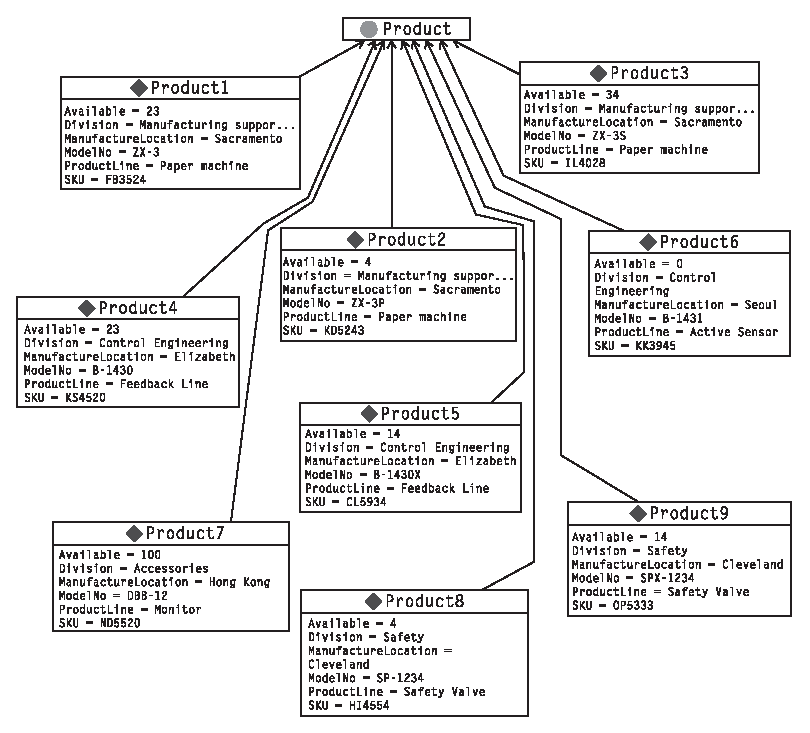
\includegraphics[width=5.0in]{media/ch3/f03-07-9780123859655.eps}
    \caption{Graphical version of the tabular data from Table~\ref{tab:ch3.12}.}
    \label{fig:ch3.7}
\end{figure}


This approach works well for examples like \emph{Shakespeare wrote
Hamlet in 1601}, in which we want to express more information about some
event or statement. It doesn't work so well in cases like
\emph{Wikipedia says Shakespeare wrote Hamlet}, in which we are
expressing information about the statement itself, \emph{Shakespeare
wrote Hamlet}. This kind of metadata about statements often takes the
form of provenance (information about the source of a statement, as in
this example), likelihood (expressed in some quantitative form like
probability, such as \emph{It is 90 percent probable that Shakespeare
wrote Hamlet}), context (specific information about a project setting in
which a statement holds, such as \emph{Kenneth Branagh played Hamlet in
the movie}), or time frame (\emph{Hamlet plays on Broadway January 11
through March 12}). In such cases, it is useful to explicitly make a
statement about a statement. This process, called explicit reification,
is supported by the W3C RDF standard with three resources called
\texttt{rdf:subject}, \texttt{rdf:predicate}, and \texttt{rdf:object}.

Let's take the example of \emph{Wikipedia says Shakespeare wrote
Hamlet}. Using the RDF standard, we can refer to a triple as follows:

\begin{lstlisting}
q:n1 rdf:subject lit:Shakespeare ; 
     rdf:predicate lit:wrote ; 
     rdf:object lit:Hamlet .
\end{lstlisting}

Then we can express the relation of Wikipedia to this statement as
follows:

\begin{lstlisting}
web:Wikipedia m:says q:n1.
\end{lstlisting}

Notice that just because we have asserted the reification triples about
\texttt{q:n1}, it is not necessarily the case that we have also asserted the
triple itself:

\begin{lstlisting}
lit:Shakespeare lit:wrote lit:Hamlet.
\end{lstlisting}

This is as it should be; after all, if an application does not trust
information from Wikipedia, then it should not behave as though that
triple has been asserted. An application that does trust Wikipedia will
want to behave as though it had.

\section{Alternatives for Serialization}
\label{serialization}
So far, we have expressed RDF triples in subject/predicate/object
tabular form or as graphs of boxes and arrows. Although these are simple
and apparent forms to display triples, they aren't always the most
compact forms, or even the most human-friendly form, to see the
relations between entities.

The issue of representing RDF in text doesn't only arise in books and
documents about RDF; it also arises when we want to publish data in RDF
on the Web. In response to this need, there are multiple ways of
expressing RDF in textual form.

\subsection{N-Triples}
\label{ntriples}

The simplest form is called \emph{N-Triples} and corresponds most directly to
the raw RDF triples. It refers to resources using their fully
unabbreviated URIs. Each URI is written between angle brackets
(\textless{} and \textgreater{}). Three resources are expressed in
subject/predicate/object order, followed by a period (.). For example,
if the namespace mfg corresponds to
\emph{http://www.WorkingOntologist.org/Examples/Chapter3/Manufacture\#}, then the first triple from Table~\ref{tab:ch3.14} is written
in N-Triples as follows:


\begin{lstlisting}
<http://www.WorkingOntologist.org/Examples/Chapter3Manufacture\#> <http://www.WorkingOntologist.org/Examples/Chapter3/Manufacture\#Product1> <http://www.WorkingOntologist.org/Examples/Chapter3/Manufacture\#Product> .
\end{lstlisting}

It is difficult to print N-Triples on a page in a book---the
serialization does not allow for new lines within a triple (as we had to
do here, to fit it in the page). An actual ntriple file has the whole
triple on a single line. The advantages of N-Triples are that they are
easy to read from a file (parse) and to write into a file for importing
and exporting.

\subsection{Turtle/N3}

In this book, we use a more compact serialization of RDF called
\emph{Turtle} which is itself a subset of a syntax called \emph{N3}. Turtle
combines the apparent display of triples from N-Triples with the
terseness of QNames. We will introduce Turtle in this section and
describe just the subset required for the current examples. We will
describe more of the language as needed for later examples. For a full
description of Turtle, see the W3C Recommendation. \footnote{https://www.w3.org/TR/turtle/}

Since Turtle uses QNames, there must be a binding between the (local)
QNames and the (global) URIs. Hence, Turtle begins with a preamble in
which these bindings are defined; for example, we can define the QNames
needed in the Challenge example with the following preamble:

\begin{lstlisting}
@prefix mfg: <http://www.WorkingOntologist.com/Examples/Chapter3/Manufacturing\#>
@prefix rdf: <http://www.w3.org/1999/02/22-rdf-syntax-ns> 
\end{lstlisting}

Once the local QNames have been defined, Turtle provides a very simple
way to express a triple by listing three resources, using QName
abbreviations, in subject/predicate/object order, followed by a period,
such as the following:

\begin{lstlisting}
mfg:Product1 rdf:type mfg:Product .
\end{lstlisting}

The final period can come directly after the resource for the object,
but we often put a space in front of it, to make it stand out visually.
This space is optional.

It is quite common (especially after importing tabular data) to have
several triples that share a common subject. Turtle provides for a
compact representation of such data. It begins with the first triple in
subject/predicate/object order, as before; but instead of terminating
with a period, it uses a semicolon (;) to indicate that another triple
with the same subject follows. For that triple, only the predicate and
object need to be specified (since it is the same subject from before).
The information in Tables~\ref{tab:ch3.13} and \ref{tab:ch3.14} about \texttt{Product1} and \texttt{Product2}
appears in Turtle as follows:

\begin{lstlisting}
mfg:Product1 rdf:type mfg:Product;
             mfg:Product\_Division "Manufacturing support"; 
             mfg:Product\_ID "1";
	     mfg:Product\_Manufacture\_Location "Sacramento";
	     mfg:Product\_ModelNo "ZX-3"; 
	     mfg:Product\_Product\_Line "Paper Machine"; 
	     mfg:Product\_SKU "FB3524";
	     mfg:Product\_Available "23" .

mfg:Product2 rdf:type mfg:Product; 
             mfg:Product\_Division "Manufacturing support"; 
	     mfg:Product\_ID "2"; 
	     mfg:Product\_Manufacture\_Location "Sacramento"; 
	     mfg:Product\_ModelNo "ZX-3P"; 
 	     mfg:Product\_Product\_Line "Paper Machine"; 
	     mfg:Product\_SKU "KD5243";
	     mfg:Product\_Available "4" .
\end{lstlisting}

When there are several triples that share both subject and predicate,
Turtle provides a compact way to express this as well so that neither
the subject nor the predicate needs to be repeated. Turtle uses a comma
(,) to separate the objects. So the fact that Shakespeare had three
children named Susanna, Judith, and Hamnet can be expressed as follows:

\begin{lstlisting}
lit:Shakespeare b:hasChild b:Susanna, b:Judith, b:Hamnet.
\end{lstlisting}

There are actually three triples represented here---namely:

\begin{lstlisting}
lit:Shakespeare b:hasChild b:Susanna. 
lit:Shakespeare b:hasChild b:Judith. 
lit:Shakespeare b:hasChild b:Hamnet.
\end{lstlisting}

Turtle provides some abbreviations to improve terseness and readability;
in this book, we use just a few of these. One of the most widely used
abbreviations is to use the word a to mean rdf:type. The motivation for
this is that in common speech, we are likely to say, ``Product1 is a
Product'' or ``Shakespeare is a playwright'' for the triples,

\begin{lstlisting}
mfg:Product1 rdf:type mfg:Product. 
lit:Shakespeare rdf:type lit:Playwright.
\end{lstlisting}

respectively. Thus we will usually write instead:

\begin{lstlisting}
mfg:Product1 a mfg:Product. 
lit:Shakespeare a lit:Playwright.
\end{lstlisting}

\subsection{RDF/XML}

While Turtle is convenient for human consumption and is more compact for
the printed page, many Web infrastructures are accustomed to
representing information in HTML or, more generally, XML. For this
reason, the W3C historically started by recommending the use of an XML
serialization of RDF called RDF/XML. The information about \texttt{Product1} and
\texttt{Product2} just shown looks as follows in RDF/XML. In this example, the
subjects (\texttt{Product1} and \texttt{Product2}) are referenced using the XML attribute
\texttt{rdf:about}; the triples with each of these as subjects appear as
subelements within these definitions. The complete details of the
RDF/XML syntax are beyond the scope of this discussion and can be found in the W3C Recommendation. \footnote{http://www.w3.org/TR/rdf-syntax-grammar/}

\begin{lstlisting}
<rdf:RDF" 
  xmlns:mfg=http://www.WorkingOntologist.com/Examples/Chapter3/Manufacturing\#"
  xmlns:rdf=http://www.w3.org/1999/02/22-rdf-syntax- ns\#">
<mfg:Product rdf:about="http://www.WorkingOntologist.com/Examples/Chapter3/Manufacturing\#Product1">
  <mfg:Available>23</mfg:Available>
  <mfg:Division>Manufacturing support</mfg:Division>
  <mfg:ProductLine>Paper machine</mfg:ProductLine>
  <mfg:SKU>FB3524</mfg:SKU>
  <mfg:ModelNo>ZX-3</mfg:ModelNo>
  <mfg:ManufactureLocation>Sacramento</mfg:ManufactureLocation>
</mfg:Product>
<mfg:Product rdf:about="http://www.WorkingOntologist.com/Examples/Chapter3/Manufacturing\#Product2">
  <mfg:SKU>KD5243</mfg:SKU>
  <mfg:Division>Manufacturing support</mfg:Division>
  <mfg:ManufactureLocation>Sacramento</mfg:ManufactureLocation>
  <mfg:Available>4</mfg:Available>
  <mfg:ModelNo>ZX-3P</mfg:ModelNo>
  <mfg:ProductLine>Paper machine</mfg:ProductLine>
</mfg:Product> 
</rdf:RDF>
\end{lstlisting}

The same information is contained in the RDF/XML form as in the Turtle,
including the declarations of the QNames for \emph{mfg:} and \emph{rdf:}. RDF/XML
includes a number of rules for determining the fully qualified URI of a
resource mentioned in an RDF/XML document. These details are quite
involved and will not be used for the examples in this book.

\subsection{JSON-LD}

A more modern way to pass data from one component to another in a Web
application is using \emph{JSON}, the Javascript Object Notation (JSON). In
order to make linked data in RDF more available to applications that use
JSON, the W3C has recommended JSON-LD, JSON for Linked Data. There is a
direct correspondence between JSON-LD and RDF triples, making JSON-LD
another serialization format for RDF.

One of the motivations for having a JSON-based serialization for RDF is
that developers who are accustomed to JSON but are not familiar with
graph data or distributed data can build applications purely in JSON,
which are nevertheless compatible with linked data.

The information about \texttt{Product1} and \texttt{Product2} looks as follows in JSONLD:

\begin{lstlisting}
{
  "@graph" : [ {
    "@id" : "mfg:Product1",
    "@type" : "mfg:Product",
    "mfg:Available" : "23",
    "mfg:Division" : "Manufacturing support",
    "mfg:ManufactureLocation" : "Sacramento",
    "mfg:ModelNo" : "ZX-3",
    "mfg:ProductLine" : "Paper machine",
    "mfg:SKU" : "FB3524"
  }, {
    "@id" : "mfg:Product2",
    "@type" : "mfg:Product",
    "mfg:Available" : "4",
    "mfg:Division" : "Manufacturing support",
    "mfg:ManufactureLocation" : "Sacramento",
    "mfg:ModelNo" : "ZX-3P",
    "mfg:ProductLine" : "Paper machine",
    "mfg:SKU" : "KD5243"
  } ],
  "@context" : {
    "rdf" : "http://www.w3.org/1999/02/22-rdf-syntax-ns#",
    "mfg" : "http://www.workingontologist.com/Examples/Chapter3/Manufacturing#"
  }
}
\end{lstlisting}


The document is organized as a \texttt{@graph} and a \texttt{@context}; the context
is like the prefix declarations in Turtle, in that it defines namespaces
abbreviations and their expansions. The graph section describes the
data, organizing it into object structures as much as possible. Each
object has an \texttt{@id}, which defines the URI of the resource (in triple
terms, the subject of each triple). The rest of the object structure is
in the same form as a JSON object, with the fields corresponding to
predicates and the values corresponding to objects.

Optionally, each object can have a \texttt{@type} declaration, which corresponds
to the \texttt{rdf:type} predicate in triples. In this case, the value is
expected to be another resource, and is interpreted as such.

JSONLD has a provision for referring to other objects as well, by using
a JSON Object syntax, specifying the identity of a referred object with
\texttt{@id}. So, if we were to say that \texttt{Product1} is a part of \texttt{Product2}, we could
say

\begin{lstlisting}
{
  "@graph" : [ {
     @id" : "mfg:Product1",
     "mfg:partOf" : { "@id" : "mfg:Product2" }
  } ]
}    
\end{lstlisting}

JSONLD provides a valuable way to exchange graph data from one
application to another, while staying entirely in a conventional
Javascript environment. Its consistency with RDF allows these
applications to smoothly integrate into a web of distributed data.

\section{BLANK NODES}

So far, we have described how RDF can represent sets of triples, in
which each subject, predicate, and object is either a source or (in the
case of the object of a triple) a literal data value. Each resource is
given an identity according to the Web standard for identity, the URI.
RDF also allows for resources that do not have any Web identity at all.
But why would we want to represent a resource that has no identity on
the Web?

Sometimes we know that something exists, and we even know some things
about it, but we don't know its identity. For instance, suppose we want
to represent the fact that Shakespeare had a mistress, whose identity
remains unknown. But we know a few things about her; she was a woman,
she lived in England, and she was the inspiration for \emph{Sonnet 78}.

It is simple enough to express these statements in RDF, but we need an
identifier for the mistress. In
Turtle, we could express them as follows:

\begin{lstlisting}
lit:Mistress1 rdf:type bio:Woman;
bio:LivedIn geo:England.
lit:Sonnet78 lit:hasInspiration lit:Mistress1.
\end{lstlisting}

But if we don't want to have an identifier for the mistress, how can we
proceed? RDF allows for a \emph{blank node}, or \emph{bnode} for short, for such a
situation. If we were to indicate a bnode with a ?, the triples would
look as follows:

\begin{lstlisting}
? rdf:type bio:Woman;
  bio:livedIn geo:England. 
lit:Sonnet78 lit:hasInspiration ?.
\end{lstlisting}

The use of the bnode in RDF can essentially be interpreted as a logical
statement, ``there exists.'' That is, in these statements we assert
``there exists a woman, who lived in England, who was the inspiration
for `Sonnet78.'''

But this notation (which does not constitute a valid Turtle expression)
has a problem: If there is
more than one blank node, how do we know which \texttt{?} references which
node? For this reason, Turtle instead includes a compact and unambiguous
notation for describing blank nodes. A blank node is indicated by
putting all the triples of which it is a subject between square brackets
({[} and {]}), so:

\begin{lstlisting}
[ rdf:type bio:Woman;
  bio:livedIn geo:England ]
\end{lstlisting}

It is customary, though not required, to leave blank space after the
opening bracket to indicate that we are acting as if there were a
subject for these triples, even though none is specified.

We can refer to this blank node in other triples by including the entire
bracketed sequence in place of the blank node. Furthermore, the
abbreviation of \texttt{a} for \texttt{rdf:type} is particularly useful in this
context. Thus, our entire statement about the mistress who inspired
``Sonnet 78'' looks as follows in Turtle:

\begin{lstlisting}
lit:Sonnet78 lit:hasInspiration [a :Woman;
             bio:livedIn geo:England].
\end{lstlisting}

This expression of RDF can be read almost directly as plain English:
that is, ``Sonnet78 has {[}as{]} inspiration a Woman {[}who{]} lived in
England.'' The identity of the woman is indeterminate. The use of the
bracket notation for blank nodes will become particularly important when
we come to describe OWL, the Web Ontology Language, since it makes very
particular use of bnodes. While RDF allows for the use of blank nodes in
many circumstances, other than the specific use of blank nodes in OWL,
their use is discouraged in general.

\subsection{Ordered information in RDF}

The children of Shakespeare appear in a certain order on the printed
page, but from the point of view of RDF, they are in no order at all;
there are just three triples, one describing the relationship between
Shakespeare and each of his children. What if we do want to specify an
ordering. How would we do it in RDF?

RDF provides a facility for ordering elements in a list format. An
ordered list can be expressed quite easily in Turtle as follows:

\begin{lstlisting}
lit:Shakespeare b:hasChild (b:Susanna b:Judith b:Hamnet).
\end{lstlisting}

This translates into the following triples, where \texttt{\_:a}, \texttt{\_:b}, and \texttt{\_:c}
are bnodes:

\begin{lstlisting}
lit:Shakespeare b:hasChild _:a.
_:a rdf:first b:Susanna.
_:a rdf:rest _:b.
_:b rdf:first b:Judith.
_:b rdf:rest _:c.
_:c rdf:rest rdf:nil.
_:c rdf:first b:Hamnet.
\end{lstlisting}

This rendition preserves the ordering of the objects but at a cost of
considerable complexity of representation. Fortunately, the Turtle
representation is quite compact, so it is not usually necessary to
remember the details of the RDF triples behind it.

\section{SUMMARY}

RDF is, first and foremost, a system for modeling data. It gives up in
compactness what it gains in flexibility. Every relationship between any
two data elements is explicitly represented, allowing for a very simple
model of merging data. There is no need to arrange the columns of tables
so that they ``match up'' or to worry about data ``missing'' from a
particular column. A relationship (expressed in a familiar form of
subject/predicate/object) is either present or it is not. Merging data
is thus reduced to a simple matter of considering all such statements
from all sources, together in a single place.

The only challenge that remains in such a system is the challenge of
identity. How do we have a global notation for the identity of any
entity? Fortunately, this problem is not unique to the RDF data model.
The infrastructure of the Web itself has the same issue and has a
standard solution: the URI. RDF borrows this solution.

Since RDF is a Web language, a fundamental consideration is the
distribution of information from multiple sources, across the Web. On
the Web, the AAA slogan holds: Anyone can say Anything about Any topic.
RDF supports this slogan by allowing any data source to refer to
resources in any name- space. Even a single triple can refer to
resources in multiple namespaces.

As a data model, RDF provides a clear specification of what has to
happen to merge information from multiple sources. It does not provide
algorithms or technology to implement those processes. These
technologies are the topic of the next chapter.

\subsection{Fundamental concepts}

The following fundamental concepts were introduced in this chapter.

\emph{\textbf{RDF (Resource Description Framework)}}---This distributes
data on the Web.

\emph{\textbf{Triple}}---The fundamental data structure of RDF. A triple
is made up of a subject, predicate, and object.

\emph{\textbf{Graph}}---A nodes-and-links structural view of RDF data.

\emph{\textbf{Merging}}---The process of treating two graphs as if they
were one.

\emph{\textbf{URI (Uniform Resource Indicator)}}---A generalization of
the URL (Uniform Resource Locator), which is the global name on the Web.

\emph{\textbf{namespace}}---A set of names that belongs to a single authority.
Namespaces allow different agents to use the same word in different
ways.

\emph{\textbf{QName}}---An abbreviated version of a URI, it is made up of a
namespace identifier and a name, separated by a colon.

\emph{\textbf{rdf:type}}---The relationship between an instance and its type.

\emph{\textbf{rdf:Property}}---The type of any property in RDF.

\emph{\textbf{Reification}}---The practice of making a statement about another
statement. It is done in RDF using

\emph{\textbf{rdf:subject}}, \emph{\textbf{rdf:predicate}}, and \emph{\textbf{rdf:object}}.

\emph{\textbf{N-Triples, Turtle, RDF/XML}}---The serialization syntaxes for
RDF.

\emph{\textbf{Blank nodes}}---RDF nodes that have no URI and thus cannot be
referenced globally. They are used to stand in for anonymous entities.
